\section{Cơ sở lý thuyết}
\subsection{Thiết kế màn chơi}
\hspace*{1cm} Một màn chơi là không gian những gì cốt lõi diễn ra trong game. Nơi này đặt ra những giới hạn cho người chơi trong việc tương tác với game. Có sự đa dạng trong từng level. Mỗi level có thể có một số điểm tương đồng, nhưng mỗi màn sẽ có những nét đặc trưng khác nhau.\\
\hspace*{1cm} Thiết kế màn chơi là một giai đoạn của quá trình phát triển trò chơi nơi các nhà phát triển tập trung tạo ra các không gian này, bao gồm các cấp độ, bản đồ và nhiệm vụ trong game. Việc thiết kế trò chơi là việc kết hợp các yếu tố cấu thành nên trải nghiệm người chơi, bao gồm cơ chế game, gameplay, cốt truyện,...\\
\hspace*{1cm} Tuy nhiên, việc thiết kế màn chơi không phải để cho có. Việc thiết kế màn chơi cần có một mục đích nào đó, ví dụ như kể chuyện, có nhân vật và phục vụ cho mục đích rõ ràng trong game. Hơn hết, người thiết kế phải tập trung vào trải nghiệm người chơi, hơn là cảm nhận bản thân. Và màn chơi phải thực sự cuốn hút và vui để mang đến trải nghiệm cho người chơi\\
\hspace*{1cm} Mục tiêu của việc thiết kế màn chơi là tạo ra các sự kiện tương tác trong môi trường game sao cho chúng mang tính thử thách người chơi. Giúp người chơi đạt được cảm giác vui sướng khi hoàn thành và có mong muốn tiếp tục gắn bó với game.\\
\subsubsection{Các bước thiết kế một màn chơi}
\hspace*{1cm} Để thiết kế màn chơi, cần tập trung vào các bước chính sau:
\begin{enumerate}
	\item \textbf{Xác định lại giới hạn dự án}\\
	Các ý tưởng có thể có rất nhiều, trông chúng có thể rất hay nhưng mà ta cũng nên nhìn lại xem giới hạn của dự án có phù hợp cho ý tưởng này không, từ đó chọn được các ý tưởng phù hợp. Nó có thể đến từ bản chất của dự án hoặc kỹ thuật. Người thiết kế màn chơi cần hiểu rõ các giới hạn này để thiết kế màn chơi sao cho hợp lý.\\
	\hspace*{1cm} Về bản chất của dự án. Điều cần phải chú ý nhất là người chơi cũng như nền tảng hiện thực. Ta cần xác định đối tượng người chơi chủ đạo của game (là trẻ em, người trưởng thành hay người cao tuổi, là nam hay nữ, có phải là mẹ bỉm sữa hay không,...) cũng như nền tảng để chơi (mobile, PC hay console). Điều này ảnh hưởng đến thời gian hoàn thiện, độ dài và độ khó của màn chơi cũng như phong cách đồ hoạ. Những dự án làm trên mobile sẽ nhanh hơn so với PC hay console. Những trò chơi nhắm đến đối tượng trẻ em thì độ dài màn chơi sẽ ngắn, độ khó cũng dễ hơn cũng như phong cách đồ hoạ cũng sẽ nhẹ đô hơn so với các game dành cho lứa tuổi người trưởng thành. Ta không thể sản xuất một tựa game có phong cách đồ hoạ máu me, hoặc chủ đề có liên quan đến chiến tranh cho đối tượng là trẻ em được.\\
	\hspace*{1cm} Về vấn đề kỹ thuật, người thiết kế màn chơi phải giữ cho game có tính nhất quán về mặt công nghệ. Người thiết kế cần biết dự án sẽ sử dụng công nghệ nào, phong cách đồ hoạ ra sao, âm thanh, nhạc nền như thế nào. Một trò chơi không thể sử dụng lẫn lộn đồ hoạ pixel và đồ hoạ vector nếu không có mục đích cụ thể, hoặc có mục đích nhưng sử dụng không hợp lý. Một trò chơi về chiến tranh thế giới thời hiện đại không thể xuất hiện các yếu tố như pháp sư, phù thuỷ hay kiếm sĩ trong các tựa game RPG được. Ngược lại, một trò chơi RPG Fantasy nếu không có yếu tố liên quan đến thế giới thực thì không thể nào có thứ gọi là súng được. Ngoài ra  Ngoài ra, hiệu ứng ánh sáng và môi trường trong game cũng là một vấn đề đáng lưu tâm. Ở các tựa game kinh dị hù doạ hoặc truy đuổi, môi trường và ánh sáng sẽ tác động nhiều đến cảm xúc của người chơi, có thể tạo cho người chơi cảm giác hồi hộp, thót tim nếu sử dụng hợp lý.\\
	\hspace*{1cm} Dưới đây là một game có thiết kế màn chơi có vấn đè về kỹ thuật, trong việc sử dụng cả pixel art, vector art và hiệu ứng ánh sáng chưa hợp lý.\\
	\begin{figure}[H]
		\centering
		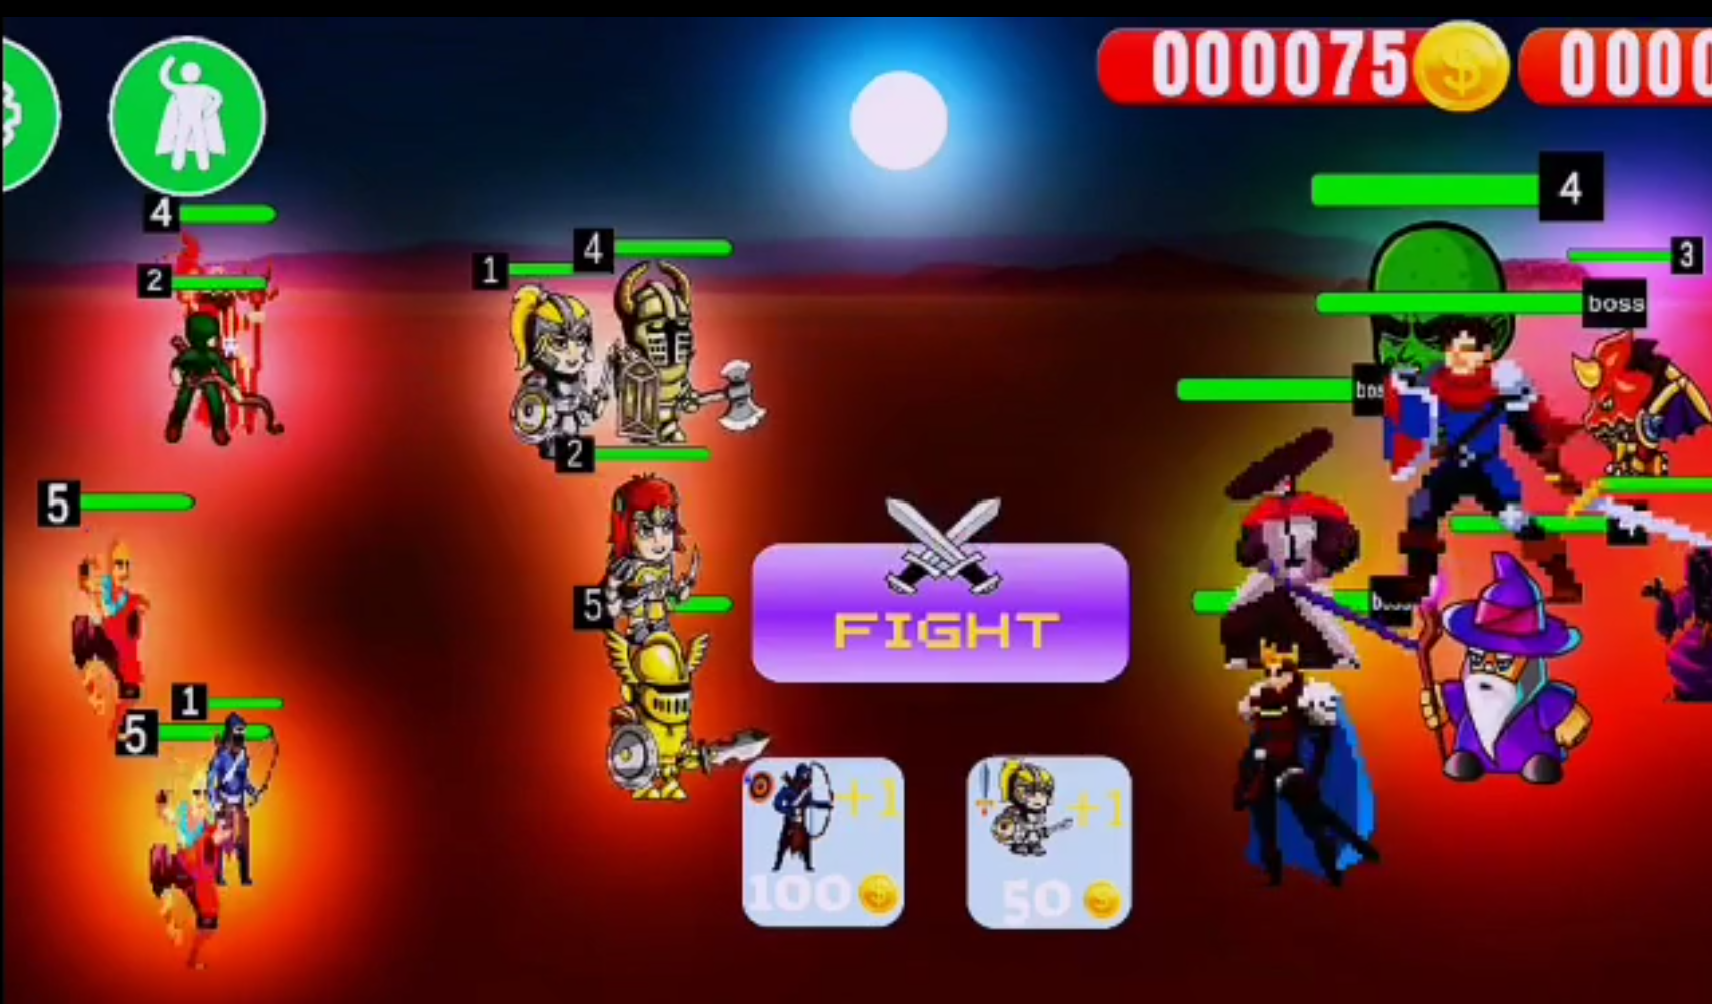
\includegraphics[width=\textwidth]{Images/AGameSuck.png}
		\vspace{0.5cm}
		\caption{Một màn chơi của game gặp vấn đề về kỹ thuật}
	\end{figure}

	\item \textbf{Lên ý tưởng và phác hoạ sơ bộ cấu trúc.}\\
	\hspace*{1cm}  Ở giai đoạn này, các thành viên khác trong dự án sẽ tiến hành lên ý tưởng và phác hoạ lên diẽn biến chính của cốt truyện cũng như xác định sơ bộ các thành phần khác của trò chơi như hình ảnh, âm thanh. Để việc thiết kế được dễ dàng hơn, người thiết kế có thể chia màn chơi thành các zone nhỏ sao cho dễ quản lý. Người thiết kế nên nghĩ đến màn chơi nếu chia thành nhiều zone sẽ ra sao và thiết kế từng zone riêng biệt để đạt hiệu suất cao và đơn giản hơn so với thiết kế toàn bộ màn chơi là một khối lớn. 
\end{enumerate}

\subsection{Ngôn ngữ truy vấn SQL}
\subsubsection{SQL là gì?}
\hspace*{1cm} SQL được viết tắt từ Structured Query Language, là một ngôn ngữ lập trình phục vụ việc lưu trữ và xử lý thông tin trong cơ sở dữ liệu quan hệ. Cơ sở dữ liệu quan hệ lưu trữ thông tin dưới dạng bảng có các hàng và cột đại diện cho những thuộc tính dữ liệu và nhiều mối quan hệ khác nhau giữa các giá trị dữ liệu. Bạn có thể sử dụng các câu lệnh SQL để lưu trữ, cập nhật, loại bỏ, tìm kiếm và truy xuất thông tin từ cơ sở dữ liệu. Bạn cũng có thể sử dụng SQL để duy trì và tối ưu hóa hiệu suất cơ sở dữ liệu.\\
\hspace*{1cm} Ngôn ngữ truy vấn có cấu trúc (SQL) là một ngôn ngữ truy vấn phổ biến thường được sử dụng trong tất cả các loại ứng dụng. Các nhà phân tích và phát triển dữ liệu tìm hiểu và sử dụng SQL do ngôn ngữ này tích hợp hiệu quả với nhiều ngôn ngữ lập trình khác nhau. Theo ANSI (American National Standards Institute - Viện Tiêu chuẩn Quốc gia Hoa Kỳ), SQL là ngôn ngữ tiêu chuẩn cho các hệ thống quản lý cơ sở dữ liệu quan hệ.
\subsubsection{SQL hoạt động như thế nào?}
\hspace*{1cm} Việc triển khai ngôn ngữ truy vấn có cấu trúc (SQL) liên quan đến một máy chủ xử lý truy vấn cơ sở dữ liệu và trả về kết quả. Quá trình SQL đi qua một số thành phần phần mềm sau:\\
\hspace*{1cm}\textbf{Trình phân tích cú pháp}\\
\hspace*{1cm}Trình phân tích cú pháp bắt đầu bằng cách token hóa hoặc thay thế một số từ trong câu lệnh SQL bằng các ký hiệu đặc biệt. Sau đó, nó sẽ kiểm tra câu lệnh để tìm kiếm những yếu tố sau:
\begin{itemize}
    \item Tính đúng đắn: Trình phân tích cú pháp xác minh rằng câu lệnh SQL tuân theo ngữ nghĩa SQL, hay các quy tắc, đảm bảo tính đúng đắn của câu lệnh truy vấn. Ví dụ: trình phân tích cú pháp kiểm tra xem lệnh SQL có kết thúc bằng dấu chấm phẩy hay không. Nếu thiếu dấu chấm phẩy, trình phân tích cú pháp sẽ trả về lỗi.
    \item Quyền hạn: Trình phân tích cú pháp cũng xác thực rằng người dùng đang chạy truy vấn có quyền cần thiết để thao tác với dữ liệu tương ứng. Ví dụ: chỉ người dùng quản trị mới có quyền xóa dữ liệu.
\end{itemize}

% \hspace*{1cm}Tính đúng đắn\\
% \hspace*{1cm}Trình phân tích cú pháp xác minh rằng câu lệnh SQL tuân theo ngữ nghĩa SQL, hay các quy tắc, đảm bảo tính đúng đắn của câu lệnh truy vấn. Ví dụ: trình phân tích cú pháp kiểm tra xem lệnh SQL có kết thúc bằng dấu chấm phẩy hay không. Nếu thiếu dấu chấm phẩy, trình phân tích cú pháp sẽ trả về lỗi.\\

% \hspace*{1cm}Quyền hạn\\
% \hspace*{1cm}Trình phân tích cú pháp cũng xác thực rằng người dùng đang chạy truy vấn có quyền cần thiết để thao tác với dữ liệu tương ứng. Ví dụ: chỉ người dùng quản trị mới có quyền xóa dữ liệu.\\
\hspace*{0.5cm}\textbf{Công cụ quan hệ}\\
\hspace*{1cm}Công cụ quan hệ, hay bộ xử lý truy vấn, tạo kế hoạch truy xuất, ghi hoặc cập nhật dữ liệu tương ứng theo cách hiệu quả nhất. Ví dụ: công cụ này kiểm tra các truy vấn tương tự, sử dụng lại các phương pháp thao tác dữ liệu trước đó hoặc tạo một phương pháp mới. Công cụ quan hệ viết kế hoạch trong mã byte, một dạng biểu diễn trung cấp của câu lệnh SQL. Cơ sở dữ liệu quan hệ sử dụng mã byte để thực hiện tìm kiếm và điều chỉnh cơ sở dữ liệu một cách hiệu quả.\\
\hspace*{1cm}\textbf{Công cụ lưu trữ}\\
\hspace*{1cm}Công cụ lưu trữ, hoặc công cụ cơ sở dữ liệu, là thành phần phần mềm xử lý mã byte và chạy câu lệnh SQL dự định. Công cụ này đọc và lưu trữ dữ liệu trong các tệp cơ sở dữ liệu trên ổ đĩa lưu trữ vật lý. Sau khi hoàn tất, công cụ lưu trữ trả về kết quả cho ứng dụng yêu cầu.
\subsubsection{Các ngôn ngữ truy vấn dữ liệu SQL}
\hspace*{1cm}Lệnh ngôn ngữ truy vấn có cấu trúc (SQL) là những từ khóa hoặc câu lệnh SQL cụ thể được các nhà phát triển sử dụng để thao tác với dữ liệu được lưu trữ trong cơ sở dữ liệu quan hệ. Bạn có thể phân loại các lệnh SQL như sau:\\
\hspace*{1cm}\textbf{Ngôn ngữ định nghĩa dữ liệu}\\
\hspace*{1cm}Ngôn ngữ định nghĩa dữ liệu (DDL) là các lệnh SQL thiết kế cấu trúc cơ sở dữ liệu. Các kỹ sư cơ sở dữ liệu sử dụng DDL để tạo và điều chỉnh các đối tượng cơ sở dữ liệu dựa trên các yêu cầu nghiệp vụ. Ví dụ: kỹ sư cơ sở dữ liệu sử dụng lệnh CREATE để tạo các đối tượng cơ sở dữ liệu như bảng, chế độ xem và chỉ mục.\\
\hspace*{1cm}\textbf{Ngôn ngữ truy vấn dữ liệu}\\
\hspace*{1cm}Ngôn ngữ truy vấn dữ liệu (DQL) bao gồm các lệnh hướng dẫn để truy xuất dữ liệu được lưu trữ trong cơ sở dữ liệu quan hệ. Các ứng dụng phần mềm sử dụng lệnh SELECT để lọc và trả về kết quả cụ thể từ một bảng SQL.\\ 
\hspace*{1cm}\textbf{Ngôn ngữ thao tác dữ liệu}\\
\hspace*{1cm}Các câu lệnh ngôn ngữ thao tác dữ liệu (DML) viết thông tin mới hoặc điều chỉnh các bản ghi hiện có trong cơ sở dữ liệu quan hệ. Ví dụ: một ứng dụng sử dụng lệnh INSERT để lưu trữ một bản ghi mới trong cơ sở dữ liệu.\\
\hspace*{1cm}\textbf{Ngôn ngữ kiểm soát dữ liệu}\\
\hspace*{1cm}Quản trị viên cơ sở dữ liệu sử dụng ngôn ngữ kiểm soát dữ liệu (DCL) để quản lý hoặc cấp quyền truy cập cơ sở dữ liệu cho người dùng khác. Ví dụ: họ có thể sử dụng lệnh GRANT để cho phép các ứng dụng nhất định thao tác với một hoặc nhiều bảng.\\
\hspace*{1cm}\textbf{Ngôn ngữ kiểm soát giao dịch}\\
\hspace*{1cm}Công cụ quan hệ sử dụng ngôn ngữ kiểm soát giao dịch (TCL) để tự động thực hiện các thay đổi đối với cơ sở dữ liệu. Ví dụ: cơ sở dữ liệu sử dụng lệnh ROLLBACK để hoàn tác một giao dịch bị lỗi.
\begin{figure}[H]
    \centering
    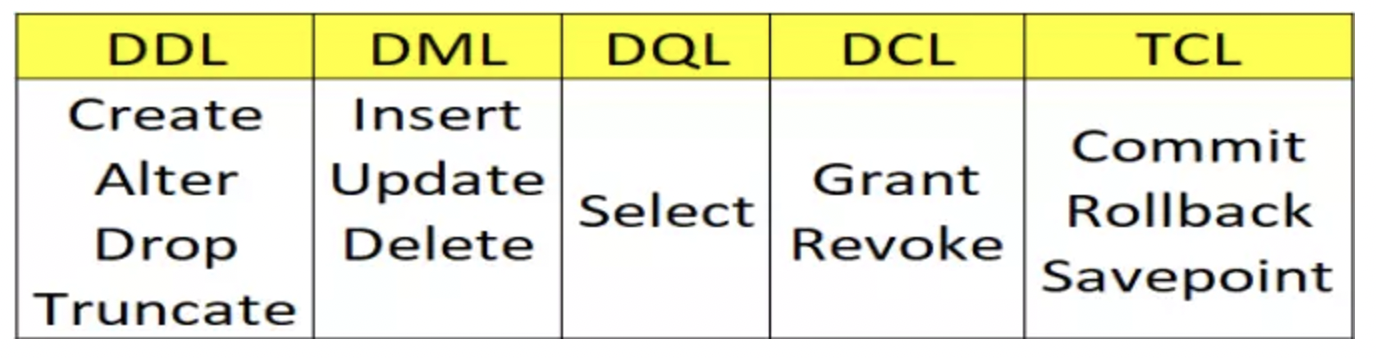
\includegraphics[width=\textwidth]{Images/lệnh SQL.png}
    \vspace{0.5cm}
    \caption{Các câu lệnh SQL cơ bản}
\end{figure}

% \subsection{Công nghệ}